%%%%%%%%%%%%%%%%%%%%%%%%%%%%%%%%%%%%%%%%%
% Wenneker Assignment
% LaTeX Template
% Version 2.0 (12/1/2019)
%
% This template originates from:
% http://www.LaTeXTemplates.com
%
% Authors:
% Vel (vel@LaTeXTemplates.com)
% Frits Wenneker
%
% License:
% CC BY-NC-SA 3.0 (http://creativecommons.org/licenses/by-nc-sa/3.0/)
% 
%%%%%%%%%%%%%%%%%%%%%%%%%%%%%%%%%%%%%%%%%

%----------------------------------------------------------------------------------------
%	PACKAGES AND OTHER DOCUMENT CONFIGURATIONS
%----------------------------------------------------------------------------------------

\documentclass[11pt]{scrartcl} % Font size

%%%%%%%%%%%%%%%%%%%%%%%%%%%%%%%%%%%%%%%%%
% Wenneker Assignment
% Structure Specification File
% Version 2.0 (12/1/2019)
%
% This template originates from:
% http://www.LaTeXTemplates.com
%
% Authors:
% Vel (vel@LaTeXTemplates.com)
% Frits Wenneker
%
% License:
% CC BY-NC-SA 3.0 (http://creativecommons.org/licenses/by-nc-sa/3.0/)
% 
%%%%%%%%%%%%%%%%%%%%%%%%%%%%%%%%%%%%%%%%%

%----------------------------------------------------------------------------------------
%	PACKAGES AND OTHER DOCUMENT CONFIGURATIONS
%----------------------------------------------------------------------------------------

\usepackage{amsmath, amsfonts, amsthm} % Math packages

\usepackage{listings} % Code listings, with syntax highlighting

\usepackage[english]{babel} % English language hyphenation

\usepackage{graphicx} % Required for inserting images
\usepackage{caption}
\graphicspath{{Figures/}{./}} % Specifies where to look for included images (trailing slash required)

\usepackage{booktabs} % Required for better horizontal rules in tables

\numberwithin{equation}{section} % Number equations within sections (i.e. 1.1, 1.2, 2.1, 2.2 instead of 1, 2, 3, 4)
\numberwithin{figure}{section} % Number figures within sections (i.e. 1.1, 1.2, 2.1, 2.2 instead of 1, 2, 3, 4)
\numberwithin{table}{section} % Number tables within sections (i.e. 1.1, 1.2, 2.1, 2.2 instead of 1, 2, 3, 4)

\setlength\parindent{0pt} % Removes all indentation from paragraphs

\usepackage{enumitem} % Required for list customisation
\setlist{noitemsep} % No spacing between list items

%----------------------------------------------------------------------------------------
%	DOCUMENT MARGINS
%----------------------------------------------------------------------------------------

\usepackage{geometry} % Required for adjusting page dimensions and margins

\geometry{
	paper=a4paper, % Paper size, change to letterpaper for US letter size
	top=2.5cm, % Top margin
	bottom=3cm, % Bottom margin
	left=3cm, % Left margin
	right=3cm, % Right margin
	headheight=0.75cm, % Header height
	footskip=1.5cm, % Space from the bottom margin to the baseline of the footer
	headsep=0.75cm, % Space from the top margin to the baseline of the header
	%showframe, % Uncomment to show how the type block is set on the page
}

%----------------------------------------------------------------------------------------
%	FONTS
%----------------------------------------------------------------------------------------

\usepackage[utf8]{inputenc} % Required for inputting international characters
\usepackage[T1]{fontenc} % Use 8-bit encoding

\usepackage{fourier} % Use the Adobe Utopia font for the document

%\usepackage[framed,numbered,autolinebreaks,useliterate]{mcode}

%----------------------------------------------------------------------------------------
%	SECTION TITLES
%----------------------------------------------------------------------------------------

\usepackage{sectsty} % Allows customising section commands

\sectionfont{\normalfont\bfseries} % \section{} styling
\subsectionfont{\normalfont\bfseries} % \subsection{} styling
\subsubsectionfont{\normalfont\itshape} % \subsubsection{} styling
\paragraphfont{\normalfont\scshape} % \paragraph{} styling

%----------------------------------------------------------------------------------------
%	HEADERS AND FOOTERS
%----------------------------------------------------------------------------------------

\usepackage{scrlayer-scrpage} % Required for customising headers and footers

\ohead*{} % Right header
\ihead*{} % Left header
\chead*{} % Centre header

\ofoot*{} % Right footer
\ifoot*{} % Left footer
\cfoot*{\pagemark} % Centre footer

% MY PACKAGES
%\usepackage[framed,numbered,autolinebreaks,useliterate]{mcode}
\usepackage{listings}
\usepackage{float}
\usepackage{amsmath}
\usepackage{tikz}
\usetikzlibrary{shapes,arrows,positioning}
\usepackage{hyperref} % Include the file specifying the document structure and custom commands

%----------------------------------------------------------------------------------------
%	TITLE SECTION
%----------------------------------------------------------------------------------------

\title{	
	\normalfont\normalsize
	\textsc{Universität Würzburg}\\ % Your university, school and/or department name(s)
	\vspace{25pt} % Whitespace
	\rule{\linewidth}{0.5pt}\\ % Thin top horizontal rule
	\vspace{20pt} % Whitespace
	{\huge Übung 5}\\ % The assignment title
	{\Large Regelabweichung, Vorfilter und Zustandsrückführung}\\
	\vspace{12pt} % Whitespace
	\rule{\linewidth}{2pt}\\ % Thick bottom horizontal rule
	\vspace{12pt} % Whitespace
}

\author{\LARGE Alexander Björk, Janis Kaltenthaler} % Your name

\date{\normalsize\today} % Today's date (\today) or a custom date

\begin{document}

\maketitle % Print the title

\tikzstyle{block} = [draw, fill=blue!20, rectangle, 
    minimum height=3em, minimum width=6em]
\tikzstyle{sum} = [draw, fill=blue!20, circle, node distance=1cm]
\tikzstyle{input} = [coordinate]
\tikzstyle{output} = [coordinate]
\tikzstyle{pinstyle} = [pin edge={to-,thin,black}]
\newcommand{\inte}{$\displaystyle \int$}

\section*{Aufgabe 5-1. Vorfilter für einen Regelkreis (3 Punkte)}
\subsection*{a)}
\subsubsection*{Steuerbarkeit}
Um die Steuerbarkeit direkt mithilfe der Übertragungsfunktion $G(s)$ bestimmen zu können, bilden wir die \textbf{Regelungsnormalform}:
\begin{align*}
	\dot{x}_R(t)&=A_Rx_R(t)+b_Ru(t),\hspace{20pt}x_R(0)=x_{R_0}\\
	y(t)&=c^T_Rx_R(t)+du(t)
\end{align*}
mit
\begin{align*}
	A_R&=-a_0=3,\hspace{10pt}&b_R=1\\
	c^T_R&=b_0-b_na_0=1,&d=0
	%\begin{bmatrix}
	%	0 & 1\\
	%	-a_0&-a_1
	%\end{bmatrix}
	%=
	%\begin{bmatrix}
	%	0 & 1\\
	%	3&-1
	%\end{bmatrix}
	%,\hspace{20pt}b_R=
	%\begin{bmatrix}
	%	 0\\
	%	1
	%\end{bmatrix}
\end{align*}
Die Regelstrecke ist somit vollständig steuerbar, da die Regelungsnormalform existiert.
\subsubsection*{Beobachtbarkeit}
Um die Beobachtbarkeit direkt mithilfe der Übertragungsfunktion $G(s)$ bestimmen zu können, bilden wir die \textbf{Beobachtungsnormalform}:
\begin{align*}
	\dot{x}_B(t)&=A_Bx_B(t)+b_Bu(t),\hspace{20pt}x_B(0)=x_{B_0}\\
	y(t)&=c^T_Bx_B(t)+du(t)
\end{align*}
mit
\begin{align*}
	A_B&=-a_0=3,\hspace{10pt}&b_B=b_0-b_na_0=1\\
	c^T_B&=1,&d=0
\end{align*}
Die Regelstrecke ist somit vollständig beobachtbar, da die Beobachtungsnormalform existiert.


\subsection*{b)}
Zur Bestimmung der statischen Verstärkung benötigen wir zunächst die Führungsübertragungsfunktion $G_W(s)=\frac{Y(s)}{W(s)}$, wobei $R(s)=0$ gilt.
\begin{align*}
	Y(s)&=E(s)K(s)G(s)\\
	Y(s)&=\bigl(W(s)-C(s)Y(s)\bigr)K(s)G(s)\\
	\Leftrightarrow\frac{Y(s)}{K(s)G(s)}&=W(s)-C(s)Y(s)\\
	\Leftrightarrow\frac{1+C(s)K(s)G(s)}{K(s)G(s)}&=\frac{W(s)}{Y(s)}\\
	\Leftrightarrow G_W(s)=\frac{Y(s)}{W(s)}&=\frac{K(s)G(s)}{1+C(s)K(s)G(s)}
\end{align*}
Durch einsetzen der gegebenen Übertragungsfunktionen erhalten wir:
\begin{align*}
	\Leftrightarrow G_W(s)=\frac{k_p\frac{1}{s-3}}{1+\frac{1}{s+5}k_p\frac{1}{s-3}}=\frac{k_p(s+5)}{s^2+2s+k_p-15}
\end{align*}
Die statische Verstärkung $k_s$ in Abhängigkeit von $k_p$ erhält man nun mit:
\begin{align*}
	\Leftrightarrow G_W(0)=k_s=\frac{k_p(0+5)}{0^2+2\cdot0+k_p-15}=\frac{5k_p}{k_p-15}
\end{align*}
$E(s)$ erhält man wie folgt, wobei $R(s)=0$ weiterhin gilt.
\begin{align*}
	E(s)&=W(s)-\hat{Y}(s)\\
	E(s)&=W(s)-E(s)K(s)G(s)C(s)\\
	%\Leftrightarrow E(s)\bigl(1+K(s)G(s)C(s)\bigr)&=W(s)\\
	\Leftrightarrow E(s)&=\frac{W(s)}{1+K(s)G(s)C(s)}
\end{align*}
Mithilfe von $E(s)$ erhält man nun die Regelabweichung $e(s)$:
\begin{align*}
	e(s)&=W(s)-Y(s)=W(s)-E(s)K(s)G(s)\\
	e(s)&=W(s)\cdot\Bigl(1-\frac{K(s)G(s)}{1+K(s)G(s)C(s)}\Bigr)\\
\end{align*}
Führt man dem Regelkreis nun den Einheitssprung zu, d.h. $W(s)=\frac{1}{s}$, erhält man für $s=0$ und durch Einsetzen der Übertragungsfunktionen die bleibende Regelabweichung.
\begin{align*}
	\lim \limits_{s \to 0}s\cdot e(s)&=\lim \limits_{s \to 0}\frac{s}{s}\cdot\Bigl(1-\frac{k_p\cdot(s+5)}{s^2+2\cdot s+k_p-15}\Bigr)=-\frac{75}{k_p-15}-4
\end{align*}
\subsection*{c)}
Um die Führungsübertragungsfunktion $G_{\hat{W}}=\frac{Y(s)}{\hat{W}(s)}$ zu bestimmen gilt $R(s)=0$. Wir verwenden die bereits in Teilaufgabe \textbf{b)} berechnete Führungsübertragungsfunktion $G_W$ und setzen nun $W(s)=V\hat{W}(s)$.
\begin{align*}
	G_{W}(s)=\frac{Y(s)}{V\hat{W}(s)}&=\frac{K(s)G(s)}{1+C(s)K(s)G(s)}\\
	\Leftrightarrow G_{\hat{W}}(s)=\frac{Y(s)}{\hat{W}(s)}&=\frac{K(s)G(s)V}{1+C(s)K(s)G(s)}
\end{align*}
\subsection*{d)}
Die Regelabweichung $e(s)$ mit dem Vorfilter $V$ ist nun:
\begin{align*}
	e(s)=V\hat{W}(s)-Y(s)=V\hat{W}(s)\cdot\Bigl(1-\frac{K(s)G(s)}{1+K(s)G(s)C(s)}\Bigl)
\end{align*}
Führt man dem Regelkreis nun den Einheitssprung zu, d.h. $\hat{W}(s)=\frac{1}{s}$, erhält man für $s=0$ und durch Einsetzen der Übertragungsfunktionen die bleibende Regelabweichung mit dem Vorfilter $V$.
\begin{align*}
	\lim \limits_{s \to 0}s\cdot e(s)&=\lim \limits_{s \to 0}V\cdot\frac{s}{s}\cdot\Bigl(1-\frac{k_p\cdot(s+5)}{s^2+2\cdot s+k_p-15}\Bigr)=-\Bigl(\frac{75}{k_p-15}-4\Bigr)\cdot V
\end{align*}
Der Vorfilter $V$ kann nun wie folgt berechnet werden um die bleibende Regelabweichung zu eliminieren:
\begin{align*}
	0&=-\Bigl(\frac{75}{k_p-15}-4\Bigr)\cdot V\\
\Leftrightarrow V&=\frac{4\cdot k_p+15}{k_p-15}
\end{align*}

\section*{Aufgabe 5-2. Drehzahlregler für einen Motor (5 Punkte)}
\subsection*{a)}
Um zu Prüfen ob der Motor vollständig steuerbar ist, verwenden wir das Steuerbarkeitskriterium von Kalman. Zuerst berechnet wir hierfür die Steuerbarkeitsmatrix $S_S$:
\begin{align*}
S_S=
\begin{bmatrix}
b &Ab
\end{bmatrix}
=
\begin{bmatrix}
0 & \frac{K_\tau}{J\cdot L}\\ \frac{1}{L} &-\frac{R^2}{L^2}
\end{bmatrix}
=
\begin{bmatrix}
0 & \frac{6\cdot 10^{-3}\frac{Nm}{A}}{8\cdot 10^{-8}kgm^2\cdot 10^{-4}H}\\ \frac{1}{10^{-4}H} &-\frac{(5\Omega)^2}{(10^{-4}H)^2}
\end{bmatrix}
\end{align*}
Der Motor ist vollständig steuerbar falls die Determinate der Steuerbarkeitsmatrix ungleich null ist:

\begin{align*}
\text{det} \hspace{3pt} S_S=-7.5\cdot 10^{12}\neq0
\end{align*}
Der Motor ist somit vollständig steuerbar.
\subsection*{b)}
Die Eigenwerte des geschlossenen Regelkreises sollen bei $\lambda_1=-10$ und $\lambda_2=-15$ liegen, was zu folgenden gewünschtem charakteristischen Polynom führt:
\begin{align*}
	\bar{p}(\lambda)=(\lambda-\bar{\lambda}_1)(\lambda-\bar{\lambda}_2)=(\lambda+10)(\lambda+15)=\lambda^2+\underbrace{25}_{\bar{a}_1}\cdot\lambda+\underbrace{150}_{\bar{a}_0}
\end{align*}
Mithilfe der Ackermann-Formel können wir nun die Zustandsrückführung $k^T$ berechnen, wobei ${S'}_S$ die letzte Zeile der Inversen der Steuerbarkeitsmatrix $S_S$ darstellt:
\begin{align*}
	k^T={S'}^T_S\bigl(\bar{a}_0I+\bar{a}_1A+A^2\bigr)=
	\begin{bmatrix}
		\frac{J\cdot L}{K_\tau} & 0
	\end{bmatrix}
	\bigl(150\cdot I+25\cdot A+A^2\bigr)=
	\begin{bmatrix}
		-\frac{275032831}{4.8\cdot 10^{10}}&-\frac{399813}{8\cdot 10^4}
	\end{bmatrix}
\end{align*}
Der Vorfilter $V$ für die Zustandsrückführung wird nun wie folgt berechnet:
\begin{align*}
	V&=-\bigl(C(A-Bk^T)^{-1}B\bigl)^{-1}=\frac{4.8\cdot 10^{10}\cdot b\cdot R-239887.8\cdot 10^6\cdot b+(4.8\cdot 10^{10}\cdot K_m-275032831)\cdot K_\tau}{4.8\cdot 10^{10}\cdot K_\tau}\\
	V&=2\cdot 10^{-7}
\end{align*}
\subsection*{c)}
Soll eine Zustandsrückführung technisch realisiert werden, müssen alle Zustandsvariablen messbar sein (oder zumindest aus den gemessenen Ausgangsgrößen rekonstruierbar sein, d.h. beobachtbar!)


\section*{Aufgabe 5-3. Reglerentwurf durch Polzuweisung für das Pendel am Wagen (5 Punkte)}
\subsection*{a)}
Die Berechnung der Eigenwerte ohne Zustandsrückführung zeigt, dass das System nicht stabil ist.
\begin{align*}
\lambda_1 &= 0 \quad\quad\quad\quad\quad\quad\hspace{3pt} \lambda_2 =  -5.5931\\
\lambda_3 &= -0.5787 \quad\quad\quad \lambda_4 = 5.5108
\end{align*}
Um das System zu stabilisieren, muss eine Zustandsrückführung durchgeführt werden, die die Pole gerade so auf die linke Halbebene verschiebt. Mit einer Verschiebung um 6 wären die neuen Pole
\begin{align*}
\lambda_1 &= -6 \quad\quad\quad\quad\quad\hspace{4pt} \lambda_2 =  -11.5931\\
\lambda_3 &= -6.5787 \quad\quad\quad \lambda_4 = -0.4892.
\end{align*}
Mit diesen Polen wäre das System stabil. Nun gilt es die Regelmatrix $K$ durch Polzuweisung zu berechnen. Dafür nehmen wir die Ackermann-Formel (auch in MATLAB implementiert). Mit den oben genannten neuen Polen, der Systemmatrix $A$ und der Eingangsmatrix $B$ ergibt sich die Regelmatrix
\begin{align*}
K=\begin{bmatrix}
-6.2750 & -15.8763 & -65.0117 & -12.0505
\end{bmatrix}.
\end{align*}

\pagebreak
\textbf{Anfangszustand (i): $x_0 = \begin{bmatrix}
0.3 & 0 & 0.15 & 0
\end{bmatrix}^T$}

Eine Simulation mit Regelmatrix $K$ zeigt, dass die Güteforderungen eingehalten wurden:
\begin{Verbatim}[frame=single]
%Wagenposition: 
ans = 
  struct with fields:
    SettlingTime: 6.4880
             Min: -9.1797e-04
         MinTime: 34.4300
             Max: 0.4143
         MaxTime: 0.3800

%Pendelwinkel:
ans = 
  struct with fields:
    SettlingTime: 0.8710
             Min: -0.0721
         MinTime: 0.3300
             Max: 0.1503
         MaxTime: 0
\end{Verbatim}

\begin{figure}[H]
	\centering
	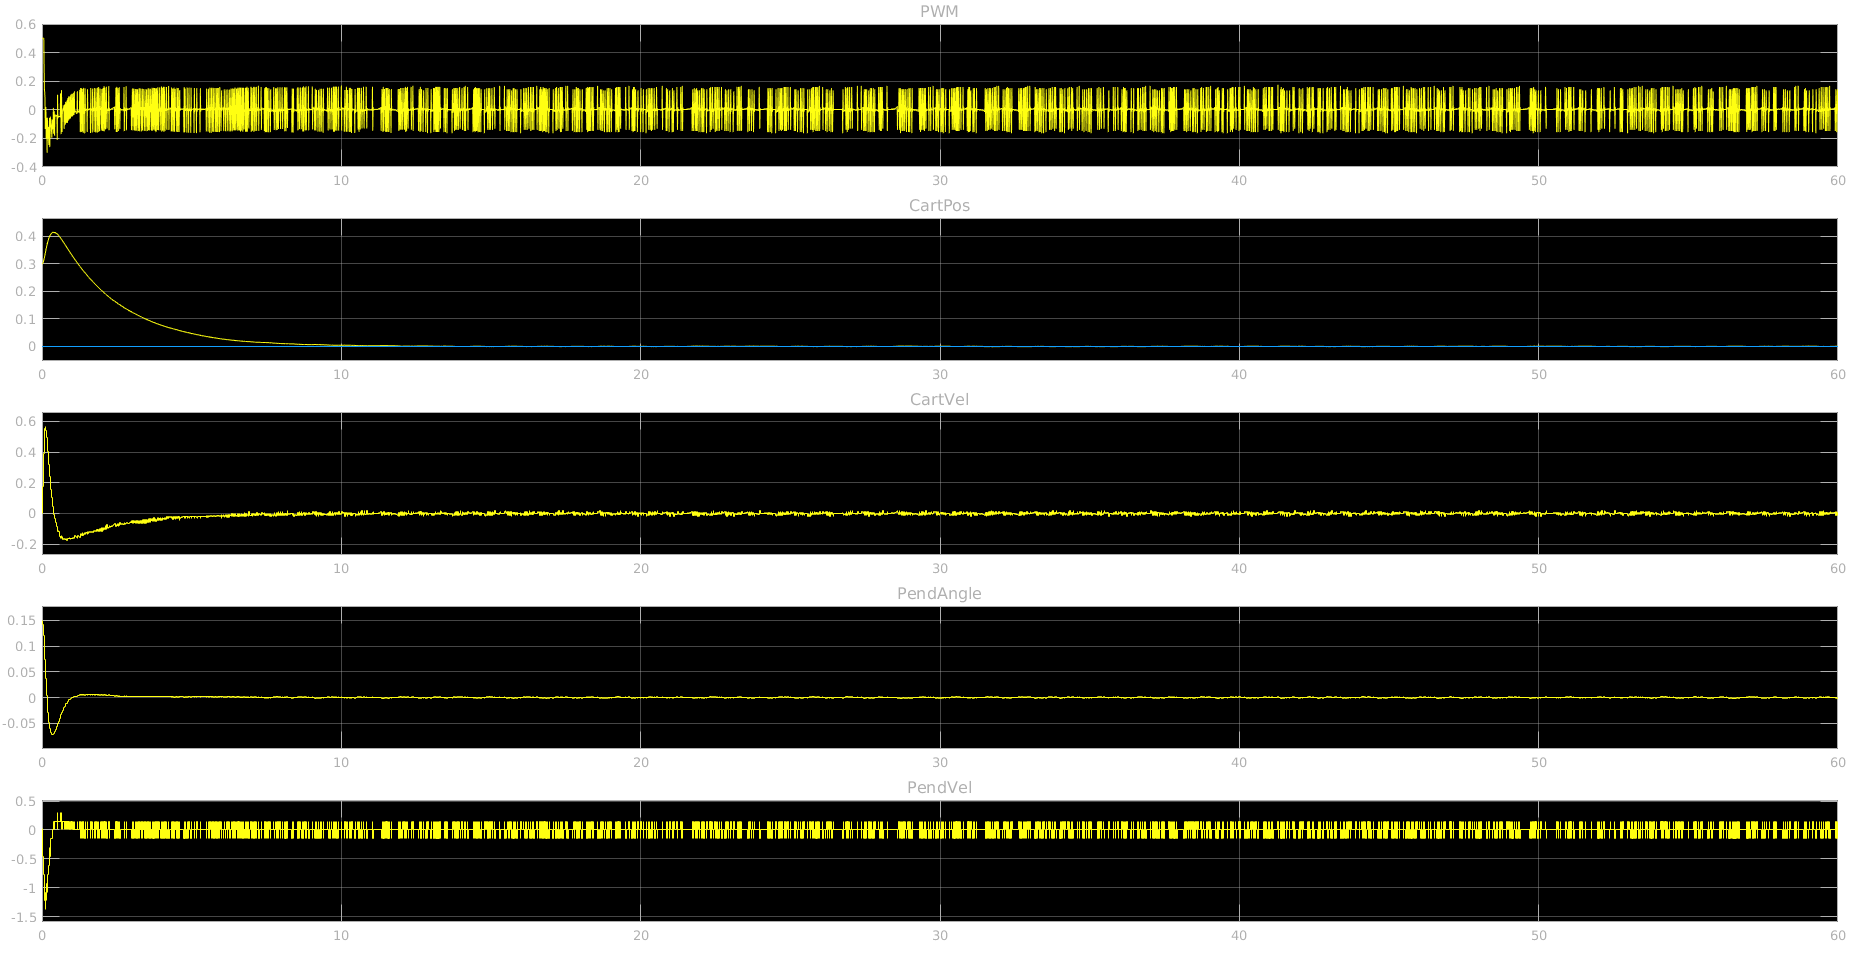
\includegraphics[width=\textwidth]{scope.png}
	\captionsetup{labelformat=empty}
	\caption{\small{Abb. 5-3.1: Scope der Pendel am Wagen Simulation mit Anfangszustand (i) und Regelmatrix K. ohne statischer Reibung}}
\end{figure}

Die Simulation zeigt, dass das System nun stabil geworden ist und die Güteforderungen eingehalten wurden. Der Wagen befindet sich zu Beginn an der Position $x=0.3$ und das Pendel bei $\theta=0.15$ (\textbf{Maximum}). Um das Pendel stabil zu halten, bewegt sich der Wagen zunächst nach rechts (dabei wird das \textbf{Maximum} bei $x=0.4143$ erreicht), um das Pendel auf eine negative Auslenkung (hier wird das Minimum von $\theta=-0.0721$ erreicht) zu bewegen, um sich anschließend nach $x=0$ zu bewegen (dies ist auch das \textbf{Minimum}). Jetzt befindet sich das System in der instabilen Ruhelage bei $x=0$ und $\theta=0$. Mit vielen kleinen Impulsen hält der Wagen nun das Pendel in dieser Ruhelage, um das Rauschen auszugleichen.

\pagebreak
\textbf{Anfangszustand (ii): $x_0 = \begin{bmatrix}
0.3 & 0 & -0.15 & 0
\end{bmatrix}^T$}

Eine Simulation mit Regelmatrix $K$ zeigt, dass auch hier die Güteforderungen eingehalten wurden:
\begin{Verbatim}[frame=single]
%Wagenposition:
ans = 
  struct with fields:
    SettlingTime: 5.4752
             Min: -0.0011
         MinTime: 34.0700
             Max: 0.3000
         MaxTime: 0

%Pendelwinkel:
ans = 
  struct with fields:
    SettlingTime: 0.9910
             Min: -0.1503
         MinTime: 0
             Max: 0.0245
         MaxTime: 0.4100
\end{Verbatim}
\begin{figure}[H]
	\centering
	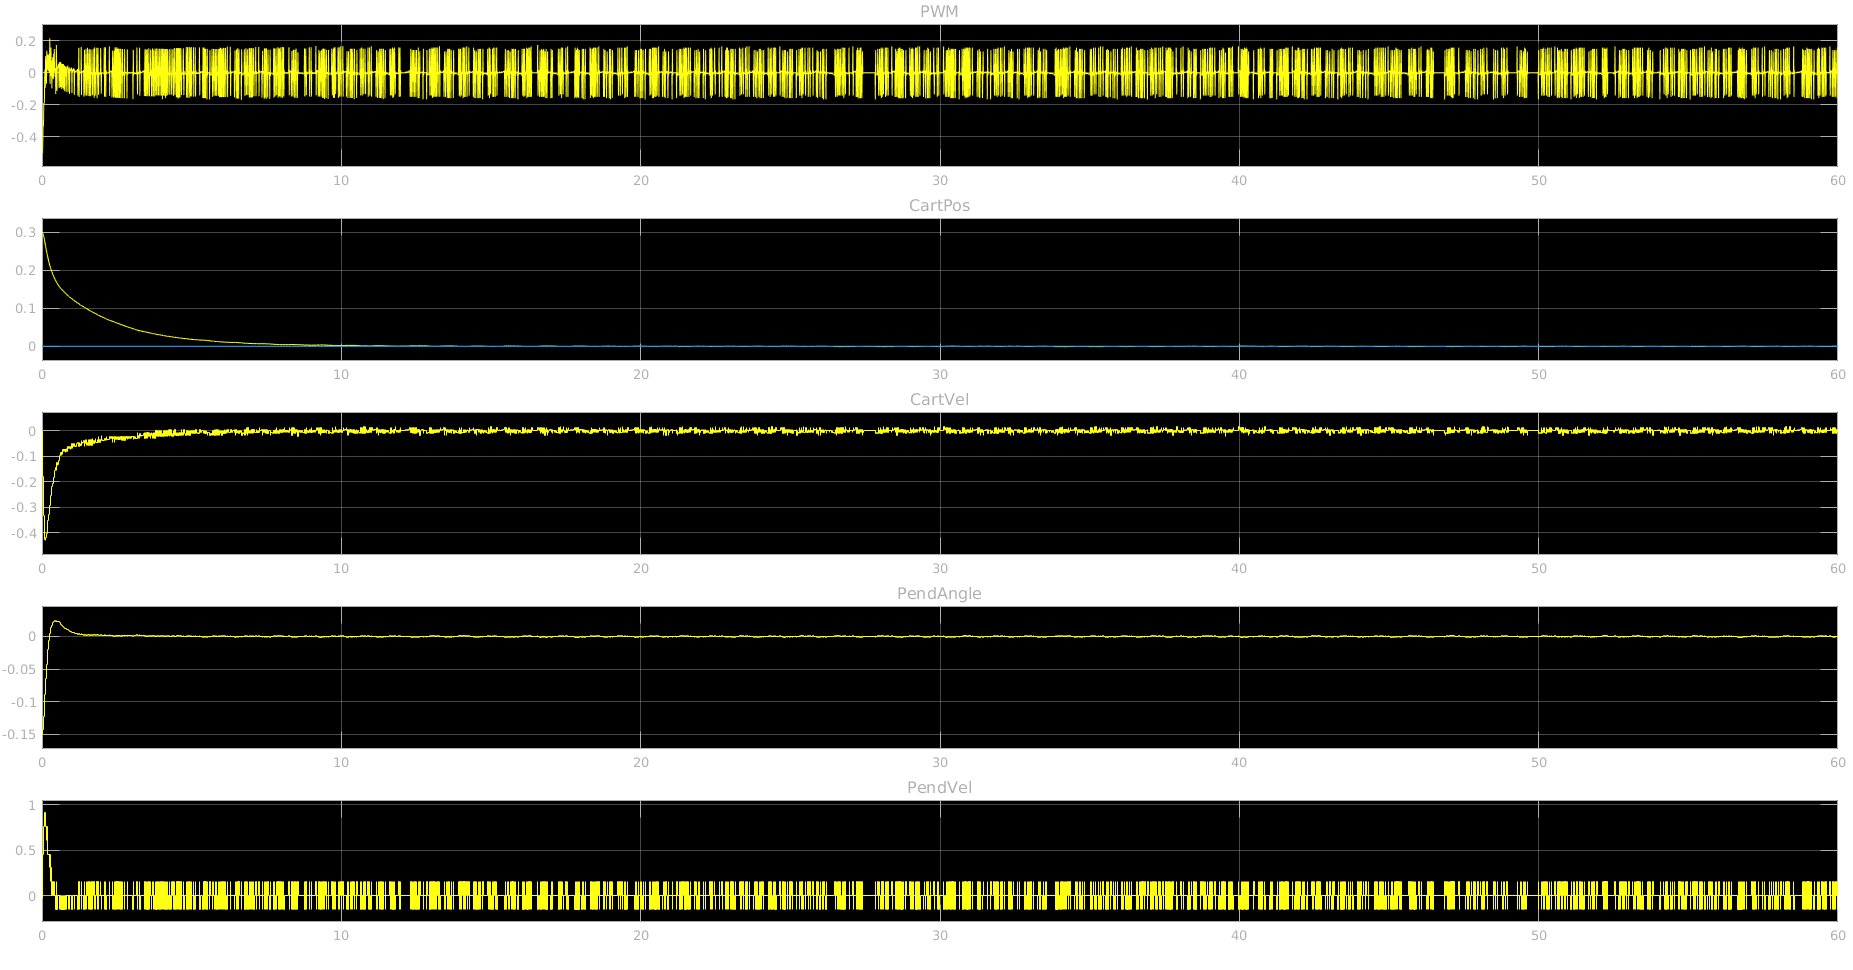
\includegraphics[width=\textwidth]{scope2.png}
	\captionsetup{labelformat=empty}
	\caption{\small{Abb. 5-3.2: Scope der Pendel am Wagen Simulation mit Anfangszustand (ii) und Regelmatrix K ohne staischer Reibung.}}
\end{figure}

Hier zeigt sich ein ähnliches Verhalten wie bei der Simulation mit Anfangszustand (i). Der Unterschied hier ist nun, dass der Wagen nicht in eine Richtung korrigieren muss, die sich vom Ursprung entfernt. Um das Pendel zu stabilisieren muss der Wagen nun nach links korrigieren. Dabei richtet sich das Pendel auf und der Wagen nähert sich dem Urpsrung. Das heißt der Wagen hat zu Simulationsbeginn sein \textbf{Maximum} bei $x=0.3$. Zum selben Zeitpunkt hat das Pendel sein \textbf{Minimum} bei $\theta=-0.15$. Nach der Korrektur der Wagenposition (die Wagenposition erreicht ihr \textbf{Minimum} bei $x=-0.0011$) erfährt der Pendelwinkel ein leichtes Überschwingen und erreicht sein \textbf{Maximum} bei $\theta=0.0245$. Das System befindet sich nun in der instabilen Ruhelage.

\subsection*{b)}
Die Pole wurden nun erneut um $1.86$ nach links verschoben. Damit ergibt sich eine Gesamtverschiebung der Pole um 7.86:
\begin{align*}
\lambda_1 &= -7.86 \quad\quad\quad\quad\quad\hspace{2pt} \lambda_2 =  -13.4531\\
\lambda_3 &= -8.4387 \quad\quad\quad\quad \lambda_4 = -2.3492.
\end{align*}
Die neue Regelmatrix ist damit
\begin{align*}
K=\begin{bmatrix}
-58.7621 & -44.3915 & -126.9155 & -23.8862
\end{bmatrix}.
\end{align*}
Die Güteforderungen an die Wagenposition konnten weiterhin eingehalten werden. Der Wagen befand sich in $\left[ -0.1019, 0.4690 \right]$. Die Güteferderungen an den Pendelwinkel jedoch konnten nicht länger eingehalten werden. Das Pendel hatte ein Minimum von $-0.3114$ und ein Maximum von $0.3605$. Während der Simulation zeigte sich, dass das System zu Beginn deutlich instabiler war als noch zuvor. Es war ebenso deutlich zu erkennen, dass der Motor an seine Grenzen von $\pm 0.5$ gelangt ist und das System gerade noch so stabil halten konnte.

\subsection*{c)}
Mit Berücksichtigung der statischen Reibung sieht man, dass das Systems schwingt. Die Wagenposition schwingt um den Nullpunkt. Selbst ohne Scope ist dies deutlich zu erkennen. Auch die Überprüfung der Güteforderungen nach der Simulation zeigt, dass sich die Wagenposition nicht beruhigt (\verb+settling time+ $\approx 60$). Der Pendelwinkel schwingt auch ganz leicht. Jedoch nicht so sehr, dass es die \verb+settling time+ beeinflusst. Das Pendel schwingt um $\pm 0.005$ mit der selben Periode wie die Schwingung der Wagenposition.

\begin{figure}[H]
	\centering
	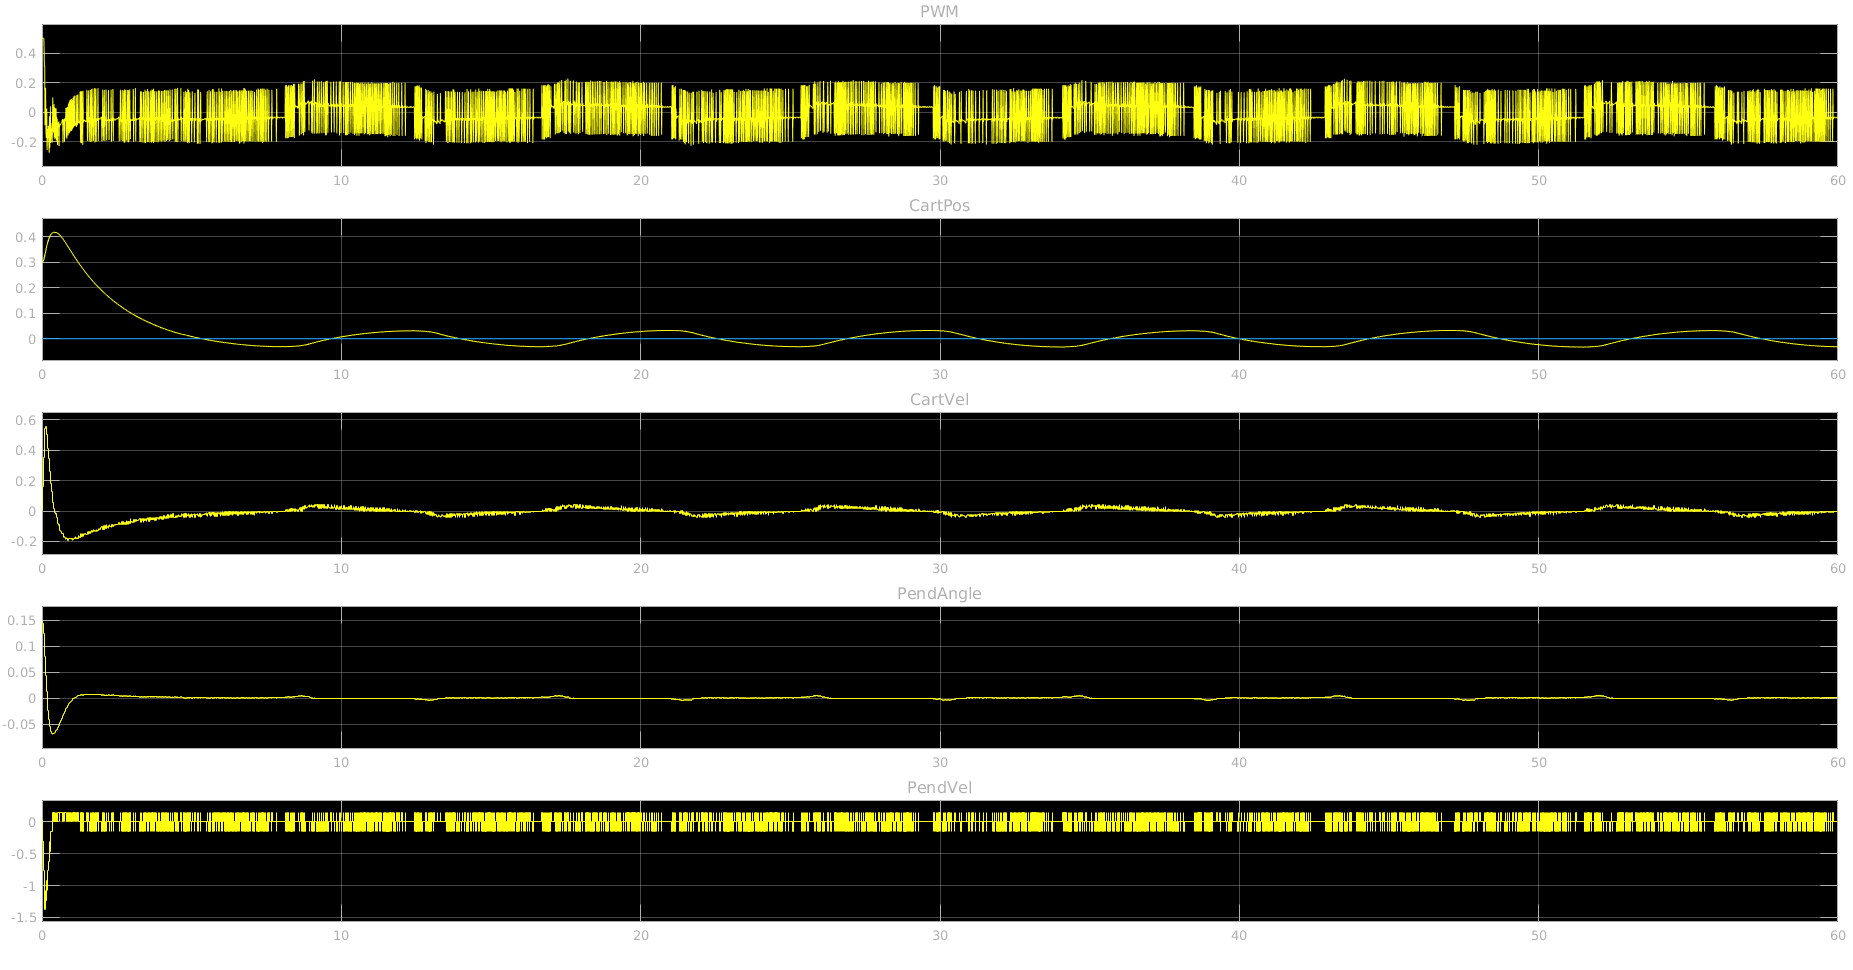
\includegraphics[width=\textwidth]{scope3.png}
	\captionsetup{labelformat=empty}
	\caption{\small{Abb. 5-3.3: Scope der Pendel am Wagen Simulation mit Anfangszustand (i) und Regelmatrix K mit statischer Reibung.}}
\end{figure}

\begin{figure}[H]
	\centering
	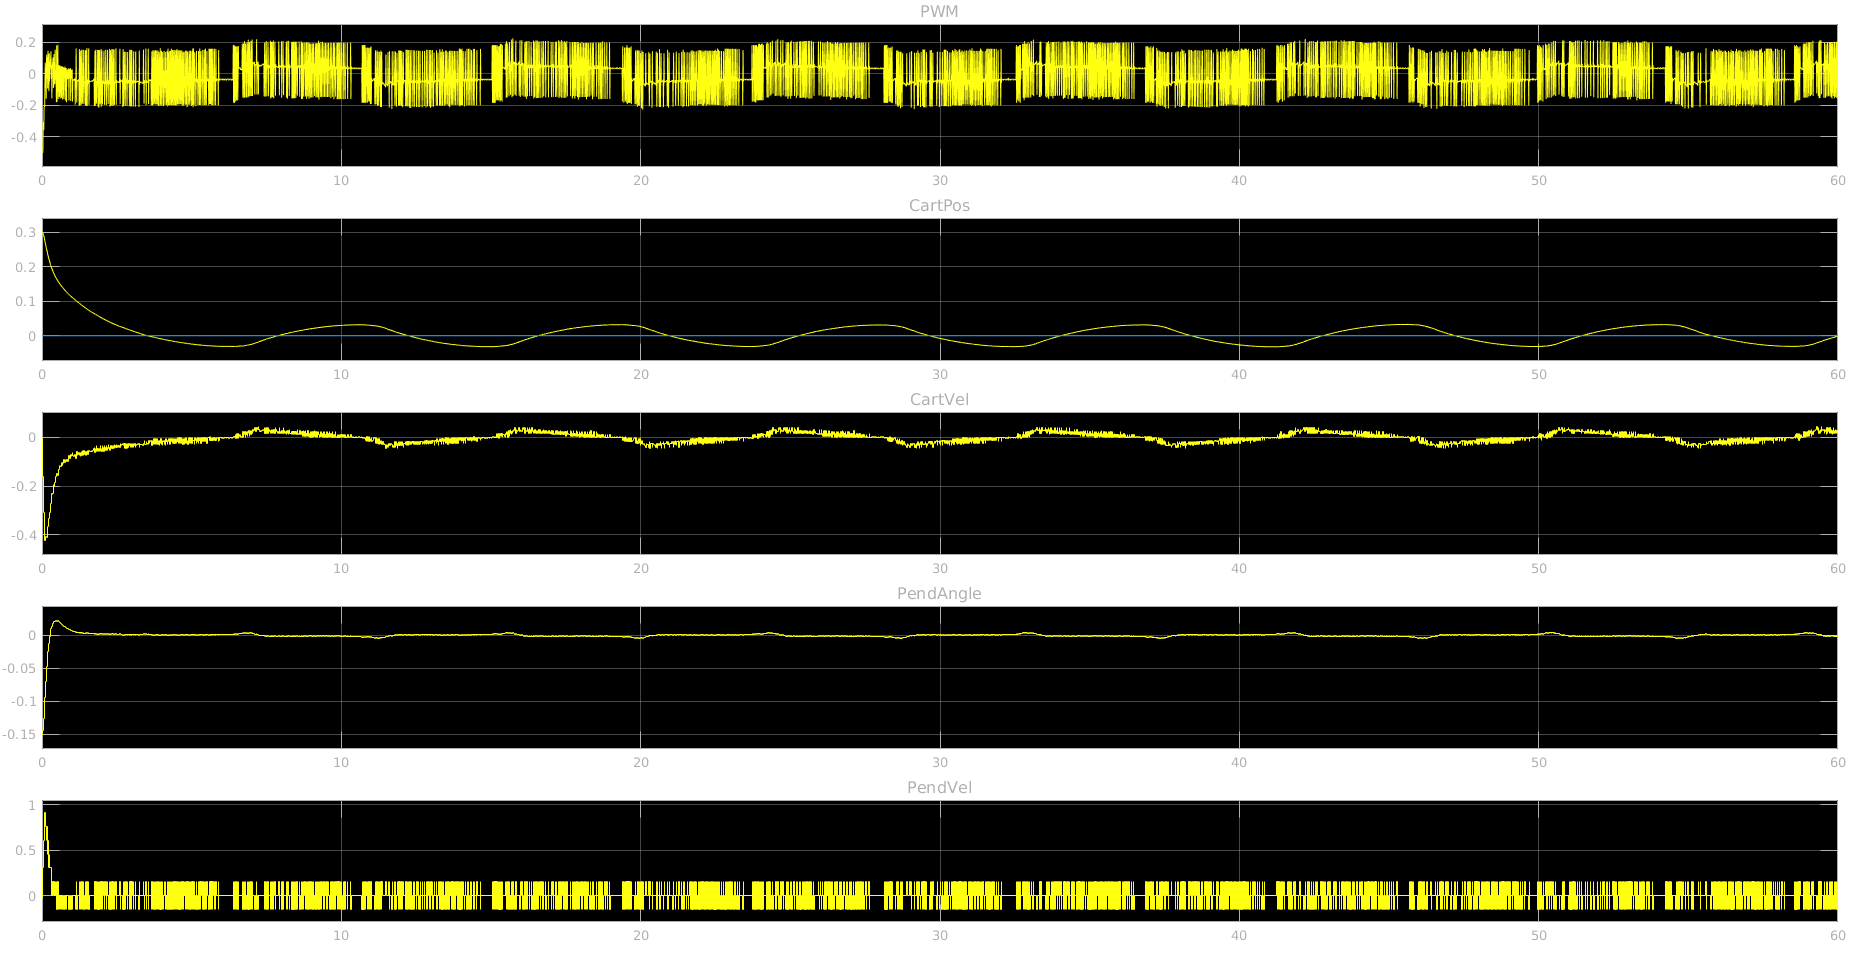
\includegraphics[width=\textwidth]{scope4.png}
	\captionsetup{labelformat=empty}
	\caption{\small{Abb. 5-3.4: Scope der Pendel am Wagen Simulation mit Anfangszustand (ii) und Regelmatrix K mit statischer Reibung.}}
\end{figure}

\end{document}
